\documentclass[conference]{IEEEtran}
\IEEEoverridecommandlockouts

% Essential Packages
\usepackage{cite}
\usepackage{amsmath,amssymb,amsfonts}
\usepackage{algorithmic}
\usepackage[final]{graphicx}
\graphicspath{{figures/}{./}}
\usepackage{textcomp}
\usepackage{xcolor}
\usepackage{booktabs}
\usepackage{multirow}
\usepackage[hyphens]{url}
\def\UrlBreaks{\do\/\do-}
\usepackage{microtype}
\usepackage{balance}
\setlength{\textfloatsep}{10pt plus 2pt minus 2pt}
\setlength{\dbltextfloatsep}{10pt plus 2pt minus 2pt}
% Times-compatible text font when compiled with XeLaTeX/Tectonic
% (pdfLaTeX, e.g. Overleaf default, uses IEEEtran's standard Times automatically).
\usepackage{iftex}
\ifXeTeX
  \usepackage{fontspec}
  \setmainfont{texgyretermes}[Extension=.otf, UprightFont=*-regular, BoldFont=*-bold, ItalicFont=*-italic, BoldItalicFont=*-bolditalic]
  \setmonofont{texgyrecursor}[Extension=.otf, UprightFont=*-regular, BoldFont=*-bold, ItalicFont=*-italic, BoldItalicFont=*-bolditalic]
\fi

\def\BibTeX{{\rm B\kern-.05em{\sc i\kern-.025em b}\kern-.08em
    T\kern-.1667em\lower.7ex\hbox{E}\kern-.125emX}}

\begin{document}

\title{Benchmarking Shallow Hybrid Quantum--Classical Models for Oral Lesion Screening: A Controlled Empirical Study}

\author{
\IEEEauthorblockN{
Ishan Narayan Shukla\IEEEauthorrefmark{1}\textsuperscript{\textsection},
Pratyaksh Ranjan\IEEEauthorrefmark{1},
Jay Karan Laxme\IEEEauthorrefmark{1},\\
Rudransh Rajveer Singh\IEEEauthorrefmark{1},
Prajjwal Patel\IEEEauthorrefmark{1},
Khoirom Motilal Singh\IEEEauthorrefmark{1}
}
\IEEEauthorblockA{\IEEEauthorrefmark{1}Department of Computer Science and Engineering\\
Indian Institute of Information Technology Manipur, Imphal, India\\
Corresponding author e-mail: ishan256022@iiitmanipur.ac.in}
\thanks{\textsuperscript{\textsection}Corresponding author: Ishan Narayan Shukla (e-mail: \mbox{ishan256022@iiitmanipur.ac.in}).}
}

\maketitle

\begin{abstract}
Although shallow variational quantum circuits and quantum kernels are frequently proposed for medical image classification, leakage-free evaluations against tuned classical baselines remain scarce. We benchmark shallow hybrid quantum--classical classifiers on the SMART-OM oral mucosa photography dataset (2,436 verified images, 328 patients, 5.9\% positive prevalence) and its clinician-annotated lesion-polygon subset (316 images, 160 patients; $k=0$ patient overlap). We evaluate four 8-qubit architectures---non-commuting fixed angle maps, fidelity quantum support vector machines (QSVM), trainable $L=2$ variational quantum classifiers (VQC), and bandwidth-tuned Havl{\'\i}{\v{c}}ek $ZZ$ maps---alongside globally entangled 16-qubit ($2^{16}$-D single-register) fixed/QSVM models and block-separable $4 \times 8$-qubit (32-D, no cross-block entanglement) extensions under matched hyperparameter budgets. All quantum models are compared against same-dimension classical controls (PCA-8/16/32 logistic and RBF-SVM, plus RFF and MLP at 8-D) and uncompressed classical references (C6: MobileNetV3, 576-D; C7: MobileNetV3 + multiscale morphology, 1,195-D). Across 5-fold patient-grouped cross-validation and held-out testing (381 full-corpus and 49 polygon test images), we find no evidence of quantum advantage. On full-corpus CV, C7 achieves $0.5776$ PR-AUC ($0.9350$ ROC-AUC), outperforming all 8-qubit models by $0.26$--$0.38$ and globally entangled 16-qubit models by $0.23$--$0.25$ PR-AUC, while matched-dimension comparisons show no statistically significant quantum gain (e.g., global 16-qubit QSVM vs.\ PCA-16 RBF-SVM: $\Delta = +0.013$, $[-0.015, +0.042]$; $4 \times 8$ QSVM vs.\ PCA-32 RBF-SVM: $\Delta = -0.008$, $[-0.021, +0.009]$). We distill five reporting standards for clinical quantum machine learning benchmarks.
\end{abstract}

\begin{IEEEkeywords}
Quantum machine learning, oral cancer screening, variational quantum circuits, quantum kernels, negative results, clinical decision support, benchmarking standards.
\end{IEEEkeywords}

\section{Introduction}
Oral cancer, predominantly oral squamous cell carcinoma (OSCC), accounts for more than 377,000 new diagnoses and 177,000 deaths annually~\cite{sung2021global}. The clinical burden falls disproportionately on low- and middle-income countries (LMICs), particularly in South Asia, where betel quid, areca nut, and tobacco use drive high incidence~\cite{sunny2019tele, piyarathne2024comprehensive}. Early identification during the phase of oral potentially malignant disorders (OPMD), such as leukoplakia and erythroplakia, substantially improves survival compared with late-stage presentation~\cite{welikala2020automated, warin2022deep}.

Computer-aided screening from smartphone oral cavity photographs has therefore gained sustained interest for frontline triage~\cite{camalan2021convolutional, welikala2020automated, smartom2026dataset}. In parallel, Noisy Intermediate-Scale Quantum (NISQ) processors~\cite{preskill2018quantum} have motivated exploratory studies of Quantum Machine Learning (QML)~\cite{biamonte2017quantum}, including Variational Quantum Classifiers (VQCs) and quantum kernel methods~\cite{cerezo2021variational, schuld2019quantum, havlicek2019supervised, abbas2021power}.

Recent benchmarking analyses, however, highlight recurrent methodological pitfalls in applied QML~\cite{bowles2024better, huang2021power, kubler2021inductive}:
\begin{enumerate}
    \item \textbf{Mismatched Baselines and Tuning Budgets:} Quantum models are frequently compared against unregularized classical models or without matched-dimension controls and equal hyperparameter budgets~\cite{bowles2024better, huang2021power}.
    \item \textbf{Patient-Level Data Leakage:} Clinical prediction guidelines such as TRIPOD~\cite{collins2015transparent} emphasize transparent validation protocols, yet systematic reviews of oral-lesion AI note inconsistent reporting of patient-disjoint splitting~\cite{warin2022deep}.
    \item \textbf{Confounded Compression Overhead:} Mapping high-dimensional image features into a small qubit register (e.g., $n=8$ qubits) introduces an information bottleneck that confounds claims about quantum expressivity unless evaluated at higher compressed dimensions as well.
    \item \textbf{Circuit and Kernel Diagnostics:} Shallow $CZ$ rings placed directly before $Z$-basis measurement commute with the readout, and untuned phase-encoded kernels can suffer severe bandwidth miscalibration~\cite{thanasilp2022subtleties, bharti2022noisy}.
\end{enumerate}

To provide a rigorous empirical reference, we evaluate shallow 8-qubit, globally entangled 16-qubit (single-register fixed/QSVM), and $4 \times 8$-qubit block-encoded (32-D) hybrid quantum--classical classifiers on the SMART-OM oral mucosa photography benchmark~\cite{smartom2026dataset}. We report: (i) 5-fold patient-grouped cross-validation across both the entire 2,436-image, 328-patient corpus and the 316-image, 160-patient clinician-annotated lesion-polygon subset; (ii) locked held-out test evaluations on both the 381-image (48-patient) full-corpus test split and the 49-image (23-patient) polygon test split; and (iii) paired patient-level bootstrap 95\% confidence intervals (CIs) throughout.

\subsection{Summary of Contributions}
\begin{itemize}
    \item \textbf{Dual-Axis Evaluation Across 8-D, 16-D, and 32-D Regimes:} We benchmark four 8-qubit paradigms---fixed non-commuting maps, fidelity QSVM, trainable $L=2$ VQC, and bandwidth-tuned $ZZ$ maps---together with globally entangled 16-qubit ($2^{16}$-D single-register) fixed/QSVM models and $4 \times 8$-qubit block-encoded (32-D, disjoint-block) counterparts against matched-dimension classical controls (PCA-8, PCA-16, and PCA-32) and uncompressed classical references (C6, C7) under matched hyperparameter tuning budgets.
    \item \textbf{Leakage-Controlled Protocol Across Scales:} All splits enforce $k=0$ patient overlap, fold-internal PCA/scaling, held-out testing on both $N=381$ (full corpus) and $N=49$ (polygon subset), and patient-level paired bootstrap 95\% CIs ($B=2,000$).
    \item \textbf{No Evidence of Advantage After Relaxing PCA-8 Compression:} On full-corpus CV (328 patients), expanding from 8-D to 32-D recovers a substantial share of the compression gap ($0.3160 \to 0.4366$ for QSVM vs.\ $0.4764$ for uncompressed C6), yet $4 \times 8$-qubit QSVM shows no gain over matched PCA-32 RBF-SVM ($0.4440$; $\Delta = -0.008$, $[-0.021, +0.009]$), and both remain below C7 ($0.5776$).
    \item \textbf{Verified Non-Commuting Entanglement and Bandwidth Diagnostics:} We verify numerically that $L=2$ $CZ$ gates modify $\langle Z_j\rangle$ ($\max|\Delta\langle Z\rangle| = 0.997$) and show via effective-rank analysis ($213.7 \to 41.7$) that untuned $ZZ$ degradation at $n=8$ is driven by bandwidth miscalibration.
    \item \textbf{Clinical QML Reporting Standards:} We distill five actionable benchmarking standards covering dual baselines, tuning parity, patient-disjoint CV, circuit non-commutation checks, and artifact reproducibility.
\end{itemize}

% -------------------------------------------------------------
\section{Related Work}

\subsection{Deep Learning in Oral Cancer and OPMD Screening}
Computer vision for oral oncology spans handcrafted colorimetric/texture descriptors and deep convolutional neural networks (CNNs). Welikala et al.~\cite{welikala2020automated} evaluated ResNet and Faster R-CNN pipelines on smartphone oral cavity photographs, showing that lesion region-of-interest (ROI) localization mitigates background interference from teeth, lips, and specular reflections. Camalan et al.~\cite{camalan2021convolutional} highlighted colorimetric and illumination shifts between benign inflammatory lesions and OPMDs. Systematic reviews of deep learning for oral lesion detection~\cite{warin2022deep} note inconsistent reporting of patient-level splitting, echoing clinical prediction standards in the TRIPOD statement~\cite{collins2015transparent}.

\subsection{Quantum Machine Learning in Medical Imaging}
Parameterized quantum circuits (PQCs) and quantum kernels~\cite{schuld2019quantum, cerezo2021variational, havlicek2019supervised} have been explored across histopathology, radiography, and physiological signals. NISQ constraints---limited qubit counts, gate errors, and finite shot budgets~\cite{bharti2022noisy, preskill2018quantum}---require compressing medical images prior to state preparation. While Caro et al.~\cite{caro2022generalization} established generalization bounds for low-depth circuits, such bounds do not imply superior predictive accuracy over regularized classical estimators.

\subsection{Critical Benchmarking and Null Results in QML}
Recent work scrutinizes claims of quantum advantage on classical datasets. Huang et al.~\cite{huang2021power} showed that classical learners with engineered features can match or exceed quantum kernels absent intrinsic quantum data structure. K{\"u}bler et al.~\cite{kubler2021inductive} analyzed quantum kernel inductive bias, while McClean et al.~\cite{mcclean2018barren} and Thanasilp et al.~\cite{thanasilp2022subtleties} characterized barren plateaus and exponential kernel concentration. Closely aligned with our methodology, Bowles et al.~\cite{bowles2024better} demonstrated across broad benchmarks that apparent quantum gains routinely vanish under fair tuning, matched controls, and proper uncertainty quantification.

% -------------------------------------------------------------
\section{Problem Formulation}

\subsection{Clinical Screening Task}
Let $\mathcal{D} = \{(x_i, y_i, p_i)\}_{i=1}^{N}$ denote oral cavity photographs with image $x_i \in \mathcal{X}$, patient identifier $p_i \in \mathcal{P}$, and binary label $y_i \in \{0, 1\}$ ($y_i = 1$: OPMD or OSCC requiring specialist referral; $y_i = 0$: normal mucosa or benign physiological variation). The goal is to rank positive cases above negatives on unseen patients. Under class imbalance, Precision-Recall Area Under the Curve (PR-AUC, average precision) is the primary metric~\cite{saito2015precision} (chance equals positive prevalence $\pi$), alongside ROC-AUC (chance $= 0.50$).

\subsection{Research Questions}
We evaluate six research questions under a locked internal protocol (recorded in the project repository prior to evaluation; no external public registry was used):
\begin{itemize}
    \item \textbf{RQ1 (Multimodal Classical Reference):} What screening performance does a regularized multimodal classical pipeline achieve?
    \item \textbf{RQ2 (Incremental Stacking Utility):} Does stacking 8-qubit predictions onto C7 yield a statistically supported increment?
    \item \textbf{RQ3 (Matched-Dimension Comparison at 8-D, 16-D, and 32-D):} At identical PCA-8, PCA-16, and PCA-32 inputs and matched tuning budgets, do shallow quantum circuits or kernels outperform classical controls?
    \item \textbf{RQ4 (Non-Commuting Entanglement Ablation):} In an $L=2$ VQC where $CZ$ gates provably alter $\langle Z_j \rangle$, does entanglement improve discrimination over a true product-state VQC?
    \item \textbf{RQ5 (Compression and Bandwidth Effects):} How do PCA dimension $d \in \{4, 8, 16, 32, 64, 128\}$ and $ZZ$ bandwidth tuning ($\gamma$) affect Gram-matrix geometry and screening accuracy?
    \item \textbf{RQ6 (Device-Calibrated Noise):} How do finite shots and IBM \texttt{FakeSherbrooke} noise affect the frozen E3 angle-encoding margin over PCA-8?
\end{itemize}

\subsection{Compression Constraints}
By the Data Processing Inequality, any lossy projection $g: \mathbb{R}^D \to \mathbb{R}^d$ satisfies $\mathcal{I}(g(X); Y) \le \mathcal{I}(X; Y)$. Because cumulative PCA explained variance measures total geometric variance rather than discriminative information directly, we isolate compression from quantum expressivity by evaluating $d=8$ (8-qubit), $d=16$ (globally entangled 16-qubit), and $d=32$ ($4 \times 8$-qubit block-encoded) regimes alongside matched classical controls.

% -------------------------------------------------------------
\section{Methodology}

\begin{figure*}[!t]
\centering
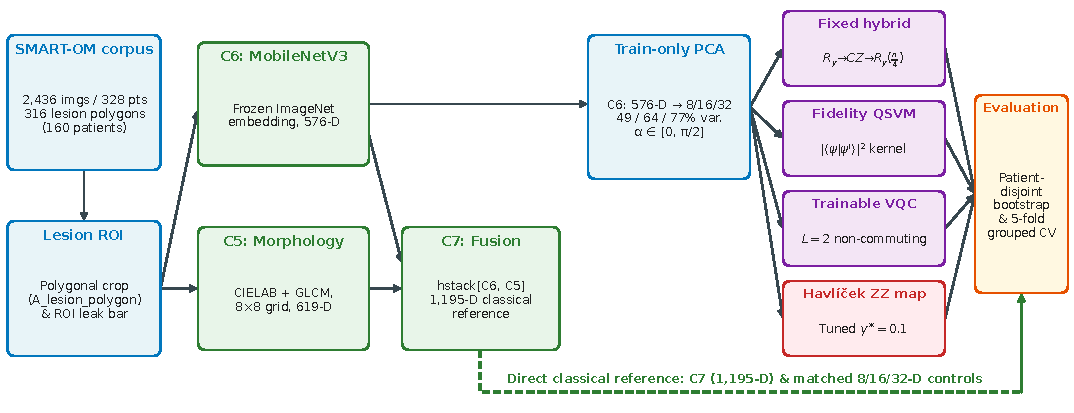
\includegraphics[width=\textwidth]{fig1_pipeline_architecture.pdf}
\caption{End-to-end evaluation architecture. Oral lesion photographs from SMART-OM (2,436 full-corpus images across 328 patients; 316 clinician-annotated lesion-polygon images across 160 patients) are processed into frozen MobileNetV3 embeddings (C6, 576-D) and multiscale morphological descriptors (C5, 619-D). Their concatenation forms the multimodal classical reference C7 (1,195-D). Independently, train-fitted PCA projects C6 (576-D) to 8-D, 16-D (globally entangled), and 32-D ($4 \times 8$ block-encoded) for shallow quantum paradigms and matched classical controls.}
\label{fig:pipeline_arch}
\end{figure*}

\subsection{Classical Representation Hierarchy (C1--C7)}
As shown in Fig.~\ref{fig:pipeline_arch} and Table~\ref{tab:candidate_definitions}, we evaluate seven classical representations: C1 (163-D CIELAB color moments, GLCM, LBP), C2/C2b (1,024-D and 256-D downsampled ROI pixels), C3 (144-D HOG), C4 (96-D rotational LBP/GLCM), C5 (619-D: C1 plus $8\times 8$ multiscale spatial grid and center-vs.-surround contrast), C6 (576-D frozen ImageNet-1K MobileNetV3-Small~\cite{howard2019searching}), and C7 (1,195-D concatenation $\text{hstack}([\text{C6}, \text{C5}])$).

\begin{table}[!t]
\caption{Classical Candidate Representations}
\label{tab:candidate_definitions}
\centering
\resizebox{\columnwidth}{!}{%
\begin{tabular}{llcc}
\toprule
\textbf{Code} & \textbf{Description / Representation Family} & \textbf{Dim ($D$)} & \textbf{Focus} \\
\midrule
C1 & Handcrafted CIELAB color \& GLCM texture & 163 & Baseline \\
C2 & Downsampled ROI pixel array & 1,024 & Raw pixel \\
C2b & Downsampled ROI pixel array & 256 & Low-dim pixel \\
C3 & Histogram of Oriented Gradients (HOG) & 144 & Edge/Margin \\
C4 & Rotational invariant LBP + GLCM texture & 96 & Micro-texture \\
C5 & C1 + $8 \times 8$ multiscale spatial grid & 619 & Spatial macro \\
C6 & MobileNetV3-Small frozen embedding & 576 & Deep semantic \\
C7 & Multimodal fusion: $\text{hstack}([\text{C6}, \text{C5}])$ & 1,195 & Multimodal ref. \\
\bottomrule
\end{tabular}%
}
\end{table}

\subsection{Input Projection and Angle Encoding}
All quantum models and matched classical controls take $\ell_2$-normalized \textbf{MobileNetV3 (C6, 576-D)} embeddings projected via fold-train-fitted PCA to $d \in \{8, 16, 32\}$ components:
\begin{equation}
\tilde{x}_i = W_d^\top \left(\frac{x_i^{\text{C6}}}{\|x_i^{\text{C6}}\|_2} - \mu_{\text{train}}\right), \quad W_d \in \mathbb{R}^{576 \times d}.
\end{equation}
Each component $\tilde{x}_{i,j}$ is mapped to $\alpha_j \in [0, \pi/2]$ via train-fold 2nd--98th percentile clipping:
\begin{equation}
\alpha_j = \text{clip}\left( \frac{\tilde{x}_{i,j} - q_{0.02, j}}{q_{0.98, j} - q_{0.02, j}} \cdot \frac{\pi}{2}, \, 0, \, \frac{\pi}{2} \right),
\end{equation}
with the $\pi/2$ upper bound selected via inner train-fold CV. Single-qubit encoding applies $U_{R_y}(\alpha) = \bigotimes_{j=1}^{8} R_y(\alpha_j)$ with $R_y(\theta) = \exp(-i\frac{\theta}{2}\sigma_y)$, and circular entanglement applies
\begin{equation}
U_{\text{ent}} = \prod_{j=1}^{8} CZ_{j, (j \bmod 8) + 1}.
\end{equation}

\subsection{Quantum Paradigms and Commutation Integrity}
Because $U_{\text{ent}}$ ($CZ$ ring) is diagonal in the $Z$ basis, it commutes with $Z$-basis observables; thus $U_{\text{ent}} U_{R_y}(\alpha)|0\rangle^{\otimes 8}$ measured in $Z$ yields $\langle Z_j\rangle = \cos(\alpha_j)$ identically with or without $CZ$. Our primary benchmark therefore uses verified non-commuting circuit topologies (Fig.~\ref{fig:circuits}). To test scaling beyond 8 qubits without relying solely on block-separable circuits, we evaluate two complementary higher-dimensional regimes: (i) \textbf{globally entangled 16-qubit} ($2^{16} = 65,536$-D single-register) fixed hybrid and fidelity QSVM circuits using a single connected 16-qubit $CZ$ ring across all 16 MobileNetV3 principal components; and (ii) \textbf{$4 \times 8$-qubit block-encoded (32-D)} versions of all four paradigms across four disjoint 8-qubit registers (entangled within each block, with \emph{no} cross-block entanglement).

\begin{figure*}[!t]
\centering
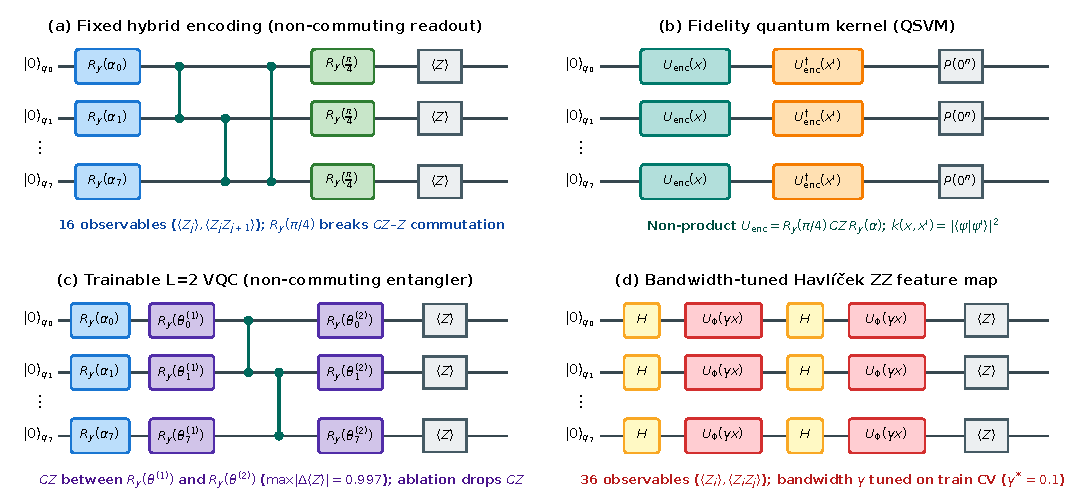
\includegraphics[width=\textwidth]{fig2_quantum_circuits.pdf}
\caption{Schematics of the four evaluated 8-qubit paradigms with verified non-commuting entanglement: (a) Fixed hybrid map $R_y(\alpha) \to CZ_{\text{ring}} \to R_y(\pi/4)$ read via 16 local/nearest-neighbor $Z$ observables; (b) Fidelity QSVM computing $k(x, x') = |\langle \psi(x) | \psi(x') \rangle|^2$ on the non-product state $U_{\text{enc}}(x)|0\rangle^{\otimes 8}$; (c) Trainable $L=2$ VQC placing $CZ_{\text{ring}}$ strictly between trainable layers $R_y(\theta^{(1)})$ and $R_y(\theta^{(2)})$ ($\max|\Delta\langle Z\rangle| = 0.997$ vs.\ true product-state ablation with zero $CZ$ gates); (d) Bandwidth-tuned Havl{\'\i}{\v{c}}ek $ZZ$ feature map $[H^{\otimes 8} U_{\Phi}(\gamma x)]^2$ read via 36 single- and two-qubit $Z$ observables. For the 32-D ($4 \times 8$) block-encoded extensions, four disjoint copies of the corresponding 8-qubit circuit process four 8-D PCA blocks in parallel with no cross-block entanglement.}
\label{fig:circuits}
\end{figure*}

\subsubsection{Fixed Non-Commuting Hybrid Map (8-Qubit and $4 \times 8$ Block-Encoded)}
Applying a basis-mixing rotation after entanglement prepares $|\psi_{\text{nc}}(\alpha)\rangle = U_{R_y}(\tfrac{\pi}{4}) U_{\text{ent}} U_{R_y}(\alpha)|0\rangle^{\otimes 8}$, reading 16 observables $\{\langle Z_j\rangle\}_{j=1}^8 \cup \{\langle Z_j Z_{(j\bmod 8)+1}\rangle\}_{j=1}^8$ into an $L_2$-regularized logistic head. The $4 \times 8$ block-encoded extension applies this map independently to four 8-D blocks (64 observables total).

\subsubsection{Fidelity-Based Quantum Kernel (8-Qubit and $4 \times 8$ Block-Encoded QSVM)}
The 8-qubit fidelity kernel computes $K_{i,j} = |\langle \psi_{\text{nc}}(x_i) | \psi_{\text{nc}}(x_j) \rangle|^2$. Its $4 \times 8$ block-encoded counterpart factorizes across the four disjoint 8-qubit blocks as $K^{(32)}(x, x') = \prod_{b=1}^{4} |\langle \psi_{\text{nc}}^{(b)}(x) | \psi_{\text{nc}}^{(b)}(x') \rangle|^2$ (no cross-block entanglement), paired with an identical dual SVM cost grid.

\subsubsection{Trainable $L=2$ VQC and True Product-State Ablation}
We train a two-layer VQC (16 circuit parameters $\boldsymbol{\theta}^{(1)}, \boldsymbol{\theta}^{(2)} \in \mathbb{R}^8$ plus a 9-parameter linear head):
\begin{equation}
|\psi(\alpha, \boldsymbol{\theta})\rangle = U_{R_y}(\boldsymbol{\theta}^{(2)})\, U_{\text{ent}}\, U_{R_y}(\boldsymbol{\theta}^{(1)})\, U_{R_y}(\alpha)|0\rangle^{\otimes 8}.
\end{equation}
Numerical checks confirm $\max|\langle Z_j\rangle_{\text{ent}} - \langle Z_j\rangle_{\text{prod}}| = 0.997$ (mean $0.285$). The ablation removes $U_{\text{ent}}$ entirely (true product state). The $4 \times 8$ block-encoded extension trains four parallel 8-qubit $L=2$ blocks (64 circuit + 33 head parameters) jointly via Adam.

\subsubsection{Bandwidth-Tuned Havl{\'\i}{\v{c}}ek $ZZ$ Feature Map}
Following~\cite{havlicek2019supervised}, we implement $\mathcal{U}_{ZZ}(x; \gamma) = \left[ U_{\Phi}(\gamma x) H^{\otimes 8} \right]^2$, with
\begin{equation}
U_{\Phi}(z) = \exp\!\left( i \sum_{j=1}^8 z_j Z_j + i \sum_{j < k} (\pi - z_j)(\pi - z_k) Z_j Z_k \right).
\label{eq:zz_unitary}
\end{equation}
We read 36 observables (8 $\langle Z_i\rangle$ + 28 pairwise $\langle Z_i Z_j\rangle$; 144 observables across four $4 \times 8$ blocks) and sweep $\gamma \in \{0.05, 0.1, 0.25, 0.5, 1.0, 2.0\}$ strictly via inner train CV, reporting Gram-matrix off-diagonal moments and effective rank $\exp(-\sum_m \tilde{\lambda}_m \ln \tilde{\lambda}_m)$.

% -------------------------------------------------------------
\section{Experimental Protocol and Integrity Controls}

\subsection{Dataset Provenance, Splits, and Prevalence Shift}
All experiments use the \textbf{SMART-OM} smartphone-based expert-annotated oral mucosa image dataset~\cite{smartom2026dataset}. From 2,469 raw images across 328 patients, quality-control auditing removed 33 degraded frames (24 severe motion blur, 3 out-of-focus, 6 specular overexposure), yielding the \textbf{verified full corpus of 2,436 images across 328 patients} (143 positive images, 5.9\% prevalence; 81 positive patients [64 OPMD, 17 OSCC] and 247 negative patients [166 normal, 81 benign variation]).

Patient-grouped hashing (\texttt{seed=42}) partitioned the 328 patients with $k=0$ overlap (Fig.~\ref{fig:patient_funnel}):
\begin{itemize}
    \item \textbf{Full Corpus (2,436 imgs / 328 pts):} Train: 1,692 images (230 patients; 104 pos.\ imgs, 57 pos.\ pts); Validation: 363 images (50 patients; 21 pos.\ imgs, 13 pos.\ pts); Held-Out Test: 381 images (48 patients; 18 pos.\ imgs, 11 pos.\ pts).
    \item \textbf{Lesion-Polygon Subset (\texttt{A\_lesion\_polygon}, 316 imgs / 160 pts):} Train: 215 images (112 patients; 103 pos., 47.9\% prev.); Validation: 52 images (25 patients; 21 pos., 40.4\% prev.); Held-Out Test: 49 images (23 patients; 18 pos., 36.7\% prev.). Positive prevalence is higher in \texttt{A\_lesion\_polygon} ($\sim 45\%$ vs.\ $5.9\%$) because clinicians preferentially draw lesion boundary polygons on suspected OPMD/OSCC and benign-variation lesions rather than normal mucosa.
\end{itemize}

\begin{figure}[!t]
\centering
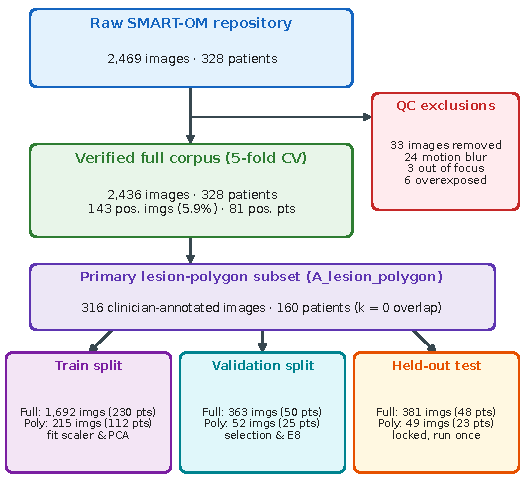
\includegraphics[width=\columnwidth]{fig8_patient_funnel.pdf}
\caption{Cohort provenance and patient-disjoint splits ($k=0$ overlap) for both the full SMART-OM corpus (2,436 images; 230/50/48 patients) and the lesion-polygon subset (316 images; 215/52/49 images across 112/25/23 patients).}
\label{fig:patient_funnel}
\end{figure}

\subsection{Matched Tuning Budgets and Statistical Protocol}
To prevent asymmetric hyperparameter tuning~\cite{bowles2024better}, Table~\ref{tab:tuning_budget} documents the exact tuning grids and parameter counts across all arms. Every scaler, PCA matrix, clipping quantile, bandwidth $\gamma$, and regularization constant $C$ is fitted strictly inside training folds. Statistical uncertainty is quantified via patient-level paired bootstrap resampling ($B=2,000$ draws). When a paired 95\% CI spans zero, we report \emph{no statistically significant difference detected} rather than claiming formal equivalence. Statevector arithmetic was cross-checked against Qiskit Aer (\texttt{qiskit 1.4.6}, \texttt{qiskit-aer 0.17.2}) to $\le 10^{-10}$.

\begin{table}[!t]
\caption{Matched Hyperparameter Tuning Budgets Across Classical and Quantum Arms (All Tuned Strictly on Inner 5-Fold Patient-Grouped Train CV)}
\label{tab:tuning_budget}
\centering
\resizebox{\columnwidth}{!}{%
\begin{tabular}{llcc}
\toprule
\textbf{Model Family} & \textbf{Input} & \textbf{Tuned Hyperparameters (Grid Size)} & \textbf{Trainable Params} \\
\midrule
C7 / C6 Logistic & 1,195 / 576-D & $C \in \{10^{-3},\dots,10^2\}$ (6) & 1,196 / 577 \\
PCA-8 / 16 / 32 Logistic & 8 / 16 / 32-D & $C \in \{10^{-3},\dots,10^2\}$ (6) & 9 / 17 / 33 \\
Fixed Q (8q / 16q / $4\times 8$q) & 8 / 16 / 32-D & $C \in \{10^{-3},\dots,10^2\}$ (6) & 17 / 33 / 65 \\
RBF-SVM (8 / 16 / 32-D) & 8 / 16 / 32-D & $C \in \{0.1, 1, 10, 100\}$ (4), auto $\gamma$ & Dual SVs \\
Fidelity QSVM (8q / 16q / $4\times 8$q) & 8 / 16 / 32-D & $C \in \{0.1, 1, 10, 100\}$ (4) & Dual SVs \\
Classical MLP Control & 8-D & Fixed 1 hidden layer (8 units, $\alpha=10^{-2}$) & 81 \\
Trainable $L=2$ VQC (8q / $4\times 8$q) & 8 / 32-D & Fixed Adam (lr $0.05$, wd $10^{-3}$) & 25 / 97 \\
Havl{\'\i}{\v{c}}ek $ZZ$ (8q / $4\times 8$q) & 8 / 32-D & $\gamma \in \{0.05,\dots,2.0\}$ (6) $\times$ $C$ (6) & 37 / 145 \\
\bottomrule
\end{tabular}%
}
\end{table}

% -------------------------------------------------------------
\section{Results}

\subsection{5-Fold Patient-Grouped CV: 8-D vs.\ 32-D Isolation (RQ1, RQ3, RQ4)}
Table~\ref{tab:grouped_cv} and Fig.~\ref{fig:leaderboard} present fold-honest 5-fold patient-grouped CV across the full 2,436-image corpus (328 patients, prevalence $0.059$) and the 316-image lesion-polygon subset (160 patients, prevalence $0.449$).

\begin{table*}[!t]
\caption{Five-Fold Patient-Grouped Cross-Validation Across Full SMART-OM Corpus ($N=2,436$, 328 Patients, Prevalence $0.059$) and Lesion-Polygon Subset ($N=316$, 160 Patients, Prevalence $0.449$) with Paired Patient-Bootstrap 95\% CIs ($B=2,000$)}
\label{tab:grouped_cv}
\centering
\resizebox{\textwidth}{!}{%
\begin{tabular}{lccccccc}
\toprule
& \multicolumn{3}{c}{\textbf{Full SMART-OM Corpus ($N=2,436$, 328 pts, prev.\ 0.059)}} & \multicolumn{3}{c}{\textbf{Lesion-Polygon Subset ($N=316$, 160 pts, prev.\ 0.449)}} & \\
\cmidrule(lr){2-4} \cmidrule(lr){5-7}
\textbf{Model / Architecture} & \textbf{OOF PR-AUC [95\% CI]} & \textbf{ROC} & \textbf{Paired $\Delta$ vs.\ C7} & \textbf{OOF PR-AUC [95\% CI]} & \textbf{ROC} & \textbf{Paired $\Delta$ vs.\ C7} & \textbf{Matched Control $\Delta$ (Full / Poly)} \\
\midrule
\textbf{C7 Classical Reference (1,195-D)} & \textbf{0.5776} [0.473, 0.688] & \textbf{0.9350} & Reference & \textbf{0.7560} [0.664, 0.840] & \textbf{0.7978} & Reference & --- \\
C6 MobileNetV3 (576-D) & 0.4764 [0.379, 0.590] & 0.9113 & --- & 0.7271 [0.636, 0.810] & 0.7762 & --- & --- \\
\midrule
\multicolumn{8}{l}{\emph{32-Dimensional Compression Isolation (PCA-32 vs.\ $4 \times 8$-Qubit Block-Encoded Quantum; No Cross-Block Entanglement)}} \\
PCA-32 Logistic Control & 0.4382 [0.358, 0.533] & 0.9006 & $-0.139$ [$-0.217, -0.064$] & 0.7069 [0.615, 0.800] & 0.7603 & $-0.049$ [$-0.106, +0.001$] & Control for Q32 Fixed / VQC / ZZ \\
Fixed Q32 ($4 \times 8$ non-comm.) & 0.4248 [0.344, 0.521] & 0.8990 & $-0.153$ [$-0.239, -0.064$] & 0.7154 [0.622, 0.805] & 0.7680 & $-0.041$ [$-0.104, +0.017$] & $-0.014$ [$-0.046, +0.023$] / $+0.009$ [$-0.021, +0.039$] \\
PCA-32 RBF-SVM Control & 0.4440 [0.355, 0.553] & 0.9136 & --- & 0.7129 [0.622, 0.802] & 0.7871 & --- & Control for Q32 QSVM \\
Fidelity Q32 QSVM ($4 \times 8$) & 0.4366 [0.353, 0.545] & 0.9140 & $-0.141$ [$-0.226, -0.052$] & 0.7169 [0.625, 0.806] & 0.7880 & $-0.039$ [$-0.094, +0.014$] & $-0.008$ [$-0.021, +0.009$] / $+0.004$ [$-0.007, +0.015$] \\
VQC Q32 $L=2$ True Product & 0.4058 [0.321, 0.503] & 0.8900 & --- & 0.6995 [0.607, 0.795] & 0.7616 & --- & Ablation control for Q32 VQC \\
VQC Q32 $L=2$ Entangled ($4 \times 8$) & 0.4105 [0.329, 0.514] & 0.9007 & $-0.167$ [$-0.247, -0.076$] & 0.6856 [0.595, 0.787] & 0.7619 & $-0.070$ [$-0.133, -0.008$] & $+0.005$ [$-0.046, +0.069$] / $-0.014$ [$-0.041, +0.016$] \\
Havl{\'\i}{\v{c}}ek Q32 $ZZ$ Tuned ($\gamma=0.1$) & 0.2437 [0.185, 0.326] & 0.8313 & $-0.334$ [$-0.431, -0.233$] & 0.6224 [0.533, 0.729] & 0.6966 & $-0.134$ [$-0.211, -0.051$] & $-0.195$ [$-0.268, -0.122$] / $-0.085$ [$-0.160, +0.003$] \\
\midrule
\multicolumn{8}{l}{\emph{16-Dimensional Globally Entangled Regime (PCA-16 vs.\ Single-Register 16-Qubit Quantum; $2^{16}$-D Connected Ring)}} \\
PCA-16 Logistic Control & 0.3540 [0.283, 0.443] & 0.8881 & --- & 0.6760 [0.586, 0.772] & 0.7649 & --- & Control for Q16 Fixed \\
Fixed Q16 (global 16q ring) & 0.3312 [0.257, 0.422] & 0.8779 & $-0.246$ [$-0.350, -0.141$] & 0.6928 [0.603, 0.791] & 0.7742 & $-0.063$ [$-0.132, +0.006$] & $-0.023$ [$-0.056, +0.007$] / $+0.017$ [$-0.017, +0.047$] \\
PCA-16 RBF-SVM Control & 0.3375 [0.264, 0.433] & 0.8800 & --- & 0.6905 [0.596, 0.789] & 0.7669 & --- & Control for Q16 QSVM \\
Fidelity Q16 QSVM (global 16q) & 0.3503 [0.274, 0.452] & 0.8891 & $-0.227$ [$-0.326, -0.123$] & 0.7013 [0.606, 0.796] & 0.7726 & $-0.055$ [$-0.126, +0.019$] & $+0.013$ [$-0.015, +0.042$] / $+0.011$ [$-0.011, +0.033$] \\
\midrule
\multicolumn{8}{l}{\emph{8-Dimensional NISQ Regime (PCA-8 vs.\ 8-Qubit Quantum)}} \\
PCA-8 Logistic Control & 0.2790 [0.213, 0.362] & 0.8634 & --- & 0.6568 [0.562, 0.762] & 0.7550 & --- & Control for Q8 Fixed \\
Fixed Q8 (non-comm.) & 0.2675 [0.200, 0.353] & 0.8526 & $-0.310$ [$-0.410, -0.201$] & 0.6882 [0.593, 0.787] & 0.7683 & $-0.068$ [$-0.139, +0.004$] & $-0.011$ [$-0.038, +0.020$] / $+0.031$ [$-0.002, +0.064$] \\
PCA-8 RBF-SVM Control & 0.3033 [0.217, 0.403] & 0.8607 & --- & 0.6889 [0.589, 0.783] & 0.7489 & --- & Control for Q8 QSVM \\
Fidelity Q8 QSVM (non-prod.) & 0.3160 [0.238, 0.415] & 0.8724 & $-0.262$ [$-0.356, -0.157$] & 0.6870 [0.583, 0.785] & 0.7623 & $-0.069$ [$-0.146, +0.002$] & $+0.013$ [$-0.046, +0.076$] / $-0.002$ [$-0.036, +0.029$] \\
VQC Q8 $L=2$ True Product & 0.2748 [0.205, 0.361] & 0.8622 & --- & 0.6618 [0.559, 0.769] & 0.7606 & --- & Ablation control for Q8 VQC \\
VQC Q8 $L=2$ Entangled ($CZ$) & 0.2619 [0.203, 0.343] & 0.8661 & $-0.316$ [$-0.410, -0.215$] & 0.6877 [0.587, 0.788] & 0.7706 & $-0.068$ [$-0.140, +0.004$] & $-0.013$ [$-0.038, +0.017$] / $+0.026$ [$-0.002, +0.050$] \\
Havl{\'\i}{\v{c}}ek Q8 $ZZ$ Tuned ($\gamma=0.1$) & 0.1929 [0.144, 0.260] & 0.7925 & $-0.385$ [$-0.488, -0.284$] & 0.6284 [0.538, 0.733] & 0.7049 & $-0.128$ [$-0.205, -0.044$] & --- \\
\bottomrule
\end{tabular}%
}
\end{table*}

\begin{figure}[!t]
\centering
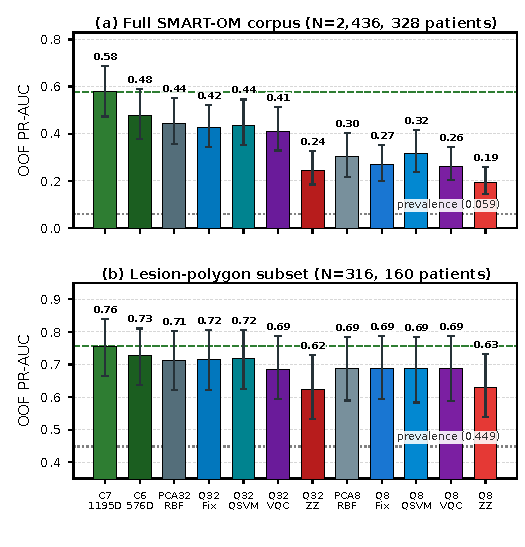
\includegraphics[width=\columnwidth]{fig3_leaderboard.pdf}
\caption{Five-fold patient-grouped CV out-of-fold PR-AUC with 95\% patient-bootstrap CIs across (a) the full 2,436-image corpus (328 patients, prevalence $0.059$) and (b) the 316-image lesion-polygon subset (160 patients, prevalence $0.449$), ordered to match Table~\ref{tab:grouped_cv}.}
\label{fig:leaderboard}
\end{figure}

Three findings stand out from Table~\ref{tab:grouped_cv}:
\begin{enumerate}
    \item \textbf{Compression Accounts for Part of the 8-D Gap, Yet Block-Separable 32-D Models Still Add No Gain:} On the full 328-patient corpus, C7 reaches $0.5776$ PR-AUC ($\sim 9.8\times$ lift over the $0.059$ prevalence baseline; ROC-AUC $0.9350$). Expanding from PCA-8 to PCA-32 narrows the gap to uncompressed C6 ($0.4764$) for classical RBF-SVM ($0.3033 \to 0.4440$), $4\times 8$ QSVM ($0.3160 \to 0.4366$), and $4\times 8$ VQC ($0.2619 \to 0.4105$), though a substantial gap remains relative to multimodal C7 ($0.5776$). Across all four 32-D paradigms, no quantum model beats its matched PCA-32 classical control: $4\times 8$ QSVM vs.\ PCA-32 RBF-SVM yields $\Delta = -0.008$ (tight 95\% CI $[-0.021, +0.009]$ on full corpus; $+0.004$, $[-0.007, +0.015]$ on polygon subset), $4\times 8$ VQC yields $-0.028$ ($[-0.074, +0.029]$) vs.\ PCA-32 logistic (used as the shared linear-head control for Fixed Q32, Q32 VQC, and Q32 $ZZ$), and $4\times 8$ $ZZ$ (linear head on 144 observables) trails PCA-32 logistic by $-0.195$ ($[-0.268, -0.122]$; note this is a linear-head rather than kernel-to-kernel comparison).
    \item \textbf{No Statistically Significant Gain at 8-D:} Across all 8-qubit paradigms, no model shows a statistically significant advantage over its matched 8-D classical control, though wider CIs (e.g., $[-0.046, +0.076]$ for Q8 QSVM vs.\ RBF-SVM) mean modest differences cannot be excluded at 8-D.
    \item \textbf{No Benefit from Non-Commuting Entanglement (RQ4):} Despite verified non-commutation ($\max|\Delta\langle Z\rangle| = 0.997$), the entangled $L=2$ VQC shows no statistically significant gain over the true product-state VQC at either 8-D ($\Delta = -0.013$, $[-0.038, +0.017]$) or 32-D ($\Delta = +0.005$, $[-0.046, +0.069]$) on the full corpus.
\end{enumerate}

\subsection{Classical Candidates and Incremental Stacking (RQ1, RQ2)}
On the \texttt{A\_lesion\_polygon} validation split ($N_{\text{val}} = 52$, 25 patients), classical candidates C1--C7 span $0.6091$ (C2b) to $0.9130$ (C7; Fig.~\ref{fig:classical_ablation}); however, because $N_{\text{val}}=52$ yields wide bootstrap CIs, we treat C1 ($0.8848$), C6 ($0.8894$), and C7 ($0.9130$) as statistically indistinguishable on validation alone and rely on multi-fold CV (Table~\ref{tab:grouped_cv}) and held-out test sets (Table~\ref{tab:test_results}) for primary inference.

In the locked E3 stacking protocol on \texttt{A\_lesion\_polygon} ($N_{\text{val}}=52$), stacking out-of-fold 8-qubit predictions onto C7 ($0.9130$) did not clear the $p < 0.05$ threshold under 200 patient-blocked column permutations (minimum possible $p = 1/201 \approx 0.005$): C7 + Fixed E3 reached $0.9302$ ($\Delta = +0.0171$, $p = 0.095$), nearly identical to classical controls C7 + RFF-16 ($0.9317$, $p = 0.070$) and C7 + PCA-8 ($0.9293$, $p = 0.080$), while C7 + QSVM ($0.9124$, $p = 0.592$), C7 + VQC ($0.8631$, $p = 0.955$), and C7 + $ZZ$ ($0.9095$, $p = 0.716$) showed negative increments. Because these stacking tests rest on the 52-image validation split with borderline $p$-values ($0.07$--$0.10$) for both quantum and classical arms, RQ2 remains underpowered and unresolved on its own.

\begin{figure}[!t]
\centering
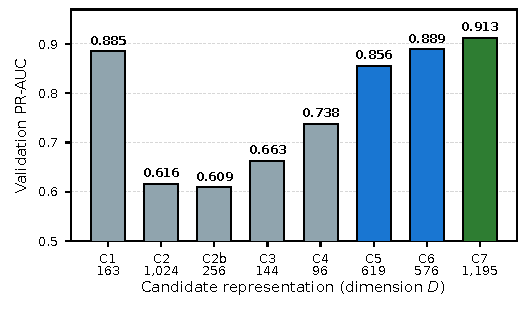
\includegraphics[width=\columnwidth]{fig7_classical_ablation.pdf}
\caption{Validation PR-AUC of the winning arm for each classical candidate (C1--C7) on \texttt{A\_lesion\_polygon} ($N_{\text{val}} = 52$, 25 patients).}
\label{fig:classical_ablation}
\end{figure}

\subsection{Dimensionality Ladder and $ZZ$ Bandwidth Diagnostics (RQ5)}
Table~\ref{tab:dim_ladder} and Fig.~\ref{fig:dim_ladder} show the PCA sweep on \texttt{A\_lesion\_polygon}. MobileNetV3 PCA-8 preserves $49.1\%$ of total PCA variance ($0.8388$ PR-AUC), peaking at $d=32$ ($76.9\%$ variance, $0.9087$) before small-sample covariance noise ($N_{\text{train}}=215$) degrades $d \ge 64$. Direct PCA on C7 is non-monotonic ($0.7384$ at $d=8$), confirming that raw PCA variance is not identical to class-discriminative information.

\begin{table}[!t]
\caption{PCA Dimensionality Ladder on \texttt{A\_lesion\_polygon} ($N_{\text{val}}=52$)}
\label{tab:dim_ladder}
\centering
\resizebox{\columnwidth}{!}{%
\begin{tabular}{ccccc}
\toprule
\textbf{Dim ($d$)} & \textbf{Qubits ($n$)} & \textbf{Cum.\ PCA Var.} & \textbf{MobileNet Val PR} & \textbf{C7 PCA Val PR} \\
\midrule
4 & 4 & 38.2\% & 0.7103 & 0.8077 \\
8 & 8 & 49.1\% & 0.8388 & 0.7384 \\
16 & 16 & 63.8\% & 0.8791 & 0.6948 \\
32 & 32 & 76.9\% & 0.9087 & 0.7325 \\
64 & 64 & 85.3\% & 0.8262 & 0.6915 \\
128 & 128 & 93.1\% & 0.7051 & 0.6938 \\
Full (576/1195) & --- & 100.0\% & 0.8894 & \textbf{0.9130} \\
\bottomrule
\end{tabular}%
}
\end{table}

\begin{figure}[!t]
\centering
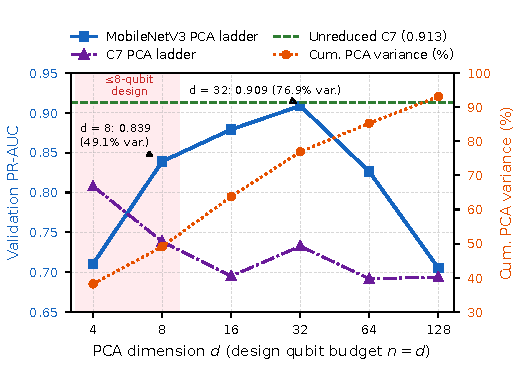
\includegraphics[width=\columnwidth]{fig4_dim_ladder.pdf}
\caption{PCA dimensionality ladder showing validation PR-AUC and cumulative PCA variance across $d \in \{4, 8, 16, 32, 64, 128\}$ on \texttt{A\_lesion\_polygon}.}
\label{fig:dim_ladder}
\end{figure}

Table~\ref{tab:zz_gram} diagnoses the $n=8$ Havl{\'\i}{\v{c}}ek $ZZ$ feature map across bandwidths $\gamma$. Untuned $\gamma=1.0$ drives the $215 \times 215$ training Gram matrix near the identity (off-diagonal mean $0.0057 \pm 0.0057$, effective rank $213.7/215$), yielding near-chance polygon test PR-AUC ($0.4165$ vs.\ $0.367$ prevalence; ROC $0.5000$). Inner train-CV tuning selects $\gamma^*=0.1$, restoring kernel overlaps ($0.2868 \pm 0.1218$, effective rank $41.7/215$) and recovering polygon test PR-AUC to $0.7226$. Thus, at $n=8$, untuned $ZZ$ degradation reflects bandwidth miscalibration rather than asymptotic exponential concentration (which remains a theoretical hazard at larger $n$); even after tuning, $ZZ$ trails C7 substantially on full-corpus CV ($0.1929$ at 8-D and $0.2437$ at 32-D vs.\ $0.5776$).

\begin{table}[!t]
\caption{Havl{\'\i}{\v{c}}ek $ZZ$ Bandwidth Sweep and Training Gram-Matrix Diagnostics ($N_{\text{train}}=215$, $n=8$ Qubits)}
\label{tab:zz_gram}
\centering
\resizebox{\columnwidth}{!}{%
\begin{tabular}{lcccc}
\toprule
\textbf{Kernel / Bandwidth ($\gamma$)} & \textbf{Train-CV PR} & \textbf{Off-Diag Mean $\pm$ SD} & \textbf{Eff.\ Rank} & \textbf{Poly Test PR} \\
\midrule
$ZZ$ ($\gamma = 0.05$) & 0.6100 & $0.5084 \pm 0.2162$ & 8.0 / 215 & --- \\
\textbf{$ZZ$ ($\gamma^* = 0.10$, CV-selected)} & \textbf{0.6185} & $\mathbf{0.2868 \pm 0.1218}$ & \textbf{41.7 / 215} & \textbf{0.7226} \\
$ZZ$ ($\gamma = 0.25$) & 0.5889 & $0.0307 \pm 0.0282$ & 191.7 / 215 & --- \\
$ZZ$ ($\gamma = 0.50$) & 0.5440 & $0.0117 \pm 0.0107$ & 210.7 / 215 & --- \\
$ZZ$ ($\gamma = 1.00$, untuned) & 0.5374 & $0.0057 \pm 0.0057$ & 213.7 / 215 & 0.4165 \\
$ZZ$ ($\gamma = 2.00$) & 0.5546 & $0.0051 \pm 0.0050$ & 214.0 / 215 & --- \\
\midrule
Fidelity QSVM (non-prod.) & 0.6925 & $0.5731 \pm 0.1565$ & 6.7 / 215 & 0.6601 \\
\bottomrule
\end{tabular}%
}
\end{table}

\subsection{Device-Calibrated Noise Attribution on Archived E3 Arm (RQ6)}
\label{sec:noise}
As a bounded noise-sensitivity check, Experiment E8 evaluated the \emph{archived frozen E3 shallow angle-encoding baseline} (separate from the non-commuting circuit protocol above; exact validation PR-AUC $0.8683$ vs.\ E3 PCA-8 $0.8388$, $\Delta_{\text{exact}} = +0.0295$) on IBM \texttt{FakeSherbrooke} (Fig.~\ref{fig:noise_robustness}): finite shots ($S=1,024$) yielded $\Delta_{\text{shots}} = +0.0453$ ($\Delta_{\text{R2}-\text{R1}} = +0.0159$), and full device noise + shots yielded $\Delta_{\text{noisy}} = +0.0391 \pm 0.0148$ ($\Delta_{\text{R3}-\text{R2}} = -0.0063$). While the point margin survives simulated device noise under E8's decision rule, the $+0.0159$ upward jump under finite shots illustrates sampling-noise sensitivity on $N_{\text{val}}=52$, and the arm fails the C7 stacking gate ($p=0.095$).

\begin{figure}[!t]
\centering
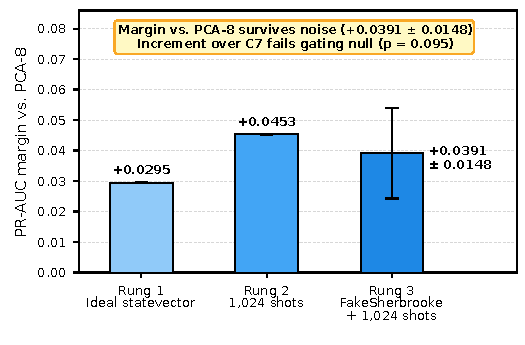
\includegraphics[width=\columnwidth]{fig5_noise_robustness.pdf}
\caption{Noise attribution ladder on IBM \texttt{FakeSherbrooke} for the archived frozen E3 shallow angle-encoding arm (RQ6).}
\label{fig:noise_robustness}
\end{figure}

\subsection{Held-Out Test Evaluation: Full Corpus ($N=381$) and Polygon Subset ($N=49$)}
Table~\ref{tab:test_results} reports locked held-out test performance on \textbf{both} the full SMART-OM test split ($N_{\text{test}}=381$ images, 48 patients, 18 positive images, prevalence $0.047$) and the polygon test split ($N_{\text{test}}=49$ images, 23 patients, 18 positive images, prevalence $0.367$; Fig.~\ref{fig:test_intervals}).

\begin{table*}[!t]
\caption{Locked Held-Out Test Performance Across Full Corpus ($N_{\text{test}}=381$, 48 Patients, Prev.\ $0.047$) and Polygon Subset ($N_{\text{test}}=49$, 23 Patients, Prev.\ $0.367$) with 95\% Patient-Bootstrap CIs ($B=2,000$)}
\label{tab:test_results}
\centering
\resizebox{\textwidth}{!}{%
\begin{tabular}{lcccccc}
\toprule
& \multicolumn{3}{c}{\textbf{Full-Corpus Held-Out Test ($N_{\text{test}}=381$, 48 pts)}} & \multicolumn{3}{c}{\textbf{Polygon Held-Out Test ($N_{\text{test}}=49$, 23 pts)}} \\
\cmidrule(lr){2-4} \cmidrule(lr){5-7}
\textbf{Model} & \textbf{Test PR-AUC [95\% CI]} & \textbf{ROC} & \textbf{Paired $\Delta$PR vs.\ C7} & \textbf{Test PR-AUC [95\% CI]} & \textbf{ROC} & \textbf{Paired $\Delta$PR vs.\ C7} \\
\midrule
C7 Reference (1,195-D) & 0.5243 [0.291, 0.804] & \textbf{0.9607} & Reference & 0.7054 [0.459, 0.933] & \textbf{0.8351} & Reference \\
\textbf{C6 (MobileNetV3, 576-D)} & \textbf{0.5592} [0.285, 0.838] & 0.9571 & --- & \textbf{0.7364} [0.488, 0.926] & 0.8118 & --- \\
\midrule
PCA-32 Logistic Control & 0.3928 [0.191, 0.692] & 0.9170 & $-0.132$ [$-0.305, +0.038$] & --- & --- & --- \\
Fixed Q32 ($4 \times 8$ block) & 0.3023 [0.131, 0.585] & 0.8797 & $-0.222$ [$-0.404, -0.038$] & --- & --- & --- \\
PCA-32 RBF-SVM Control & 0.5343 [0.253, 0.781] & 0.9434 & --- & --- & --- & --- \\
Fidelity Q32 QSVM ($4 \times 8$) & 0.5197 [0.253, 0.762] & 0.9411 & $-0.005$ [$-0.201, +0.154$] & --- & --- & --- \\
VQC Q32 $L=2$ Entangled ($4 \times 8$) & 0.4311 [0.213, 0.752] & 0.9279 & $-0.093$ [$-0.308, +0.129$] & --- & --- & --- \\
VQC Q32 $L=2$ True Product & 0.4540 [0.217, 0.709] & 0.9164 & --- & --- & --- & --- \\
$ZZ$ Q32 Tuned ($\gamma=0.1$) & 0.2132 [0.078, 0.486] & 0.8470 & $-0.311$ [$-0.519, -0.110$] & --- & --- & --- \\
\midrule
PCA-16 Logistic Control & 0.3550 [0.175, 0.630] & 0.8994 & --- & 0.6813 [0.436, 0.879] & 0.7581 & --- \\
PCA-16 RBF-SVM Control & 0.4453 [0.217, 0.707] & 0.9291 & --- & 0.6726 [0.415, 0.879] & 0.7742 & --- \\
Fixed Q16 (global 16q ring) & 0.2662 [0.125, 0.514] & 0.8759 & $-0.258$ [$-0.436, -0.083$] & 0.7062 [0.464, 0.883] & 0.7581 & $+0.001$ [$-0.182, +0.181$] \\
Fidelity Q16 QSVM (global 16q) & 0.4024 [0.194, 0.674] & 0.9117 & $-0.122$ [$-0.341, +0.092$] & 0.7987 [0.579, 0.941] & 0.8620 & $+0.093$ [$-0.119, +0.305$] \\
\midrule
PCA-8 Logistic Control & 0.2102 [0.097, 0.426] & 0.8491 & --- & 0.6005 [0.359, 0.807] & 0.6810 & --- \\
PCA-8 RBF-SVM Control & 0.3109 [0.121, 0.590] & 0.8924 & --- & 0.6520 [0.395, 0.871] & 0.7204 & --- \\
Fixed Q8 (non-comm.) & 0.2124 [0.084, 0.456] & 0.8414 & $-0.312$ [$-0.521, -0.120$] & 0.5783 [0.345, 0.809] & 0.6810 & $-0.127$ [$-0.297, +0.053$] \\
Fidelity Q8 QSVM & 0.2613 [0.116, 0.543] & 0.8880 & $-0.263$ [$-0.465, -0.056$] & 0.6601 [0.416, 0.869] & 0.7384 & $-0.045$ [$-0.217, +0.111$] \\
VQC Q8 $L=2$ Entangled & 0.2051 [0.089, 0.443] & 0.8584 & $-0.319$ [$-0.521, -0.144$] & 0.6223 [0.346, 0.853] & 0.7025 & $-0.083$ [$-0.264, +0.077$] \\
VQC Q8 $L=2$ True Product & 0.2021 [0.095, 0.407] & 0.8525 & --- & 0.6263 [0.380, 0.828] & 0.6935 & --- \\
$ZZ$ Q8 Tuned ($\gamma=0.1$) & 0.1272 [0.054, 0.330] & 0.7567 & $-0.397$ [$-0.629, -0.161$] & 0.7226 [0.478, 0.895] & 0.7348 & $+0.017$ [$-0.184, +0.174$] \\
$ZZ$ Q8 Untuned ($\gamma=1.0$) & --- & --- & --- & 0.4165 [0.226, 0.649] & 0.5000 & $-0.289$ [$-0.492, -0.096$] \\
\midrule
ROI Area Leak-Bar & --- & --- & --- & 0.3417 [0.196, 0.564] & 0.4337 & $-0.364$ [$-0.572, -0.148$] \\
\bottomrule
\end{tabular}%
}
\end{table*}

\begin{figure}[!t]
\centering
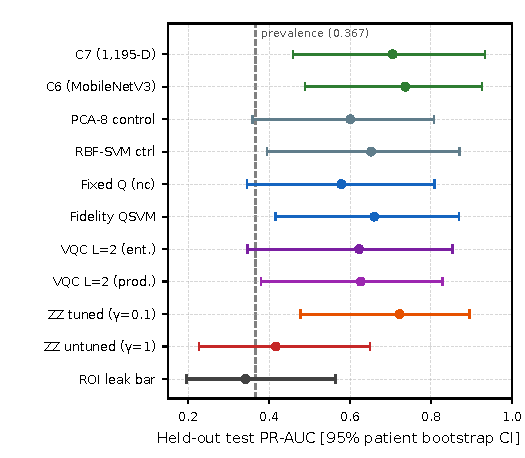
\includegraphics[width=\columnwidth]{fig6_test_intervals.pdf}
\caption{Held-out polygon test PR-AUC ($N_{\text{test}}=49$, 23 patients) with 95\% patient-bootstrap CIs for the 8-qubit suite, C6, C7, matched 8-D controls, and the geometric ROI-area leak bar (globally entangled 16-qubit and 32-D test results appear in Table~\ref{tab:test_results}).}
\label{fig:test_intervals}
\end{figure}

On the 381-image full-corpus test set, \textbf{C6 MobileNetV3 outperforms C7 on PR-AUC} ($0.5592$ vs.\ $0.5243$, $>11\times$ lift over prevalence $0.047$) while \textbf{C7 leads on ROC-AUC} ($0.9607$ vs.\ $0.9571$) and full-corpus CV PR-AUC ($0.5776$ vs.\ $0.4764$). A similar pattern holds on the 49-image polygon test set (C6 PR-AUC $0.7364$ vs.\ C7 $0.7054$; C7 ROC-AUC $0.8351$ vs.\ C6 $0.8118$). Because both held-out test splits contain only $18$ positive images ($11$ positive patients), 5-fold patient-grouped CV (Table~\ref{tab:grouped_cv}) carries the primary statistical weight, and individual test-set point fluctuations should not be interpreted as definitive evidence. On the 381-image full-corpus test, globally entangled 16-qubit Fixed Q16 ($0.2662$) trails PCA-16 logistic ($0.3550$; paired $\Delta = -0.089$, $[-0.192, -0.018]$, computed from the same test scores as Table~\ref{tab:test_results}), whereas on 5-fold CV the two show no statistically significant difference ($\Delta = -0.023$, $[-0.056, +0.007]$), reflecting wider finite-sample test variance; global 16-qubit QSVM ($0.4024$) shows no gain over PCA-16 RBF-SVM ($0.4453$, $\Delta = -0.043$ $[-0.101, +0.009]$). On the small 49-image polygon test, global Q16 QSVM reaches $0.7987$ vs.\ PCA-16 RBF-SVM $0.6726$ ($\Delta = +0.126$ $[-0.016, +0.261]$, CI spanning zero)—further illustrating small-sample volatility compared with the tight full-corpus CV bound ($+0.013$ $[-0.015, +0.042]$). Every 8-qubit model trails C7 by $0.26$--$0.40$ PR-AUC on full-corpus test, and $4\times 8$ block-encoded 32-D models show no gain over matched PCA-32 controls. On the 49-image polygon test, C7 significantly exceeds the geometric ROI-area leak bar ($\Delta\text{PR} = +0.364$, $[+0.148, +0.572]$).

\subsection{Cross-Modal Secondary Check: PTB-XL ECG Screening}
As a high-power secondary check, we evaluated an analogous patient-disjoint fusion pipeline on the 12-lead ECG PTB-XL benchmark ($N = 21,837$ records across 18,885 patients; standard folds 1--8 train, 9 validation, 10 test)~\cite{wagner2020ptb}. Specifically, 8-D PCA-compressed ECG features were passed through an 8-qubit $ZZ$ quantum feature map (36 observables) and stacked with a 1D-CNN and gradient-boosted tabular model, compared against a same-shape degree-2 polynomial classical fusion baseline ($0.9404$ test ROC-AUC). The paired test ROC-AUC difference was $\Delta = +0.00064$ (95\% patient-bootstrap CI $[-0.00049, +0.00175]$). While a degree-2 polynomial is a modest classical comparator for 8-D features, failing to surpass even it rules out ROC-AUC increments exceeding $+0.002$ for that specific fusion pipeline.

% -------------------------------------------------------------
\section{Discussion}

\subsection{Isolating Compression from Quantum Expressivity}
Evaluating both 8-qubit and $4 \times 8$-qubit block-encoded (32-D) suites across all four paradigms disentangles compression loss from quantum expressivity:
\begin{enumerate}
    \item \textbf{Compression Penalty at 8 Qubits:} Truncating MobileNetV3 to 8 dimensions discards $50.9\%$ of total PCA variance, depressing PR-AUC by $0.26$--$0.38$ on the full corpus.
    \item \textbf{No Gain Even at 32 Dimensions:} Relaxing compression to PCA-32 recovers a substantial share of the gap toward uncompressed C6 ($0.4764$ CV), yet all four $4 \times 8$ block-encoded models still fail to outperform matched PCA-32 classical baselines (most tightly bounded by Q32 QSVM vs.\ PCA-32 RBF-SVM: $\Delta = -0.008$, $[-0.021, +0.009]$ on CV), and C7 retains an additional margin ($0.5776$ CV) from C5 morphological features.
    \item \textbf{Entanglement, Bandwidth, and Statistical Power:} Verified non-commuting $L=2$ entanglement provides no statistically significant gain over a true product-state VQC at either 8-D or 32-D, and untuned $ZZ$ maps at $n=8$ fail primarily due to bandwidth miscalibration (effective rank $213.7 \to 41.7$ after tuning $\gamma^*=0.1$). We note candidly that wide CIs on the 8-D comparisons and 49-image polygon test set cannot exclude small-to-moderate quantum gains; our strongest bounds come from $4 \times 8$ QSVM on full-corpus CV and the PTB-XL secondary check.
\end{enumerate}

\subsection{Recommended Reporting Standards for Clinical QML}
Building on Bowles et al.~\cite{bowles2024better} and TRIPOD~\cite{collins2015transparent}, we recommend five standards for future clinical QML evaluations:
\begin{enumerate}
    \item \textbf{Dual Baselines \& Compression Isolation:} Report both matched-dimension classical controls (at multiple compressed widths, e.g., $d=8$ and $d=32$) and an uncompressed classical reference.
    \item \textbf{Tuning-Budget Parity:} Document identical inner-CV tuning grids and parameter budgets for quantum and classical arms (Table~\ref{tab:tuning_budget}).
    \item \textbf{Patient-Disjoint Multi-Fold CV ($k=0$):} Enforce patient grouping across splits, folds, and bootstraps, reporting exact patient and image counts for every subset and explaining any prevalence enrichment.
    \item \textbf{Circuit Non-Commutation \& Kernel Diagnostics:} Verify numerically that entanglers alter measured observables and report Gram-matrix statistics and bandwidth sweeps.
    \item \textbf{Cautious Statistical Inference:} Use paired patient-bootstrap CIs and distinguish underpowered null intervals from tight bounds.
\end{enumerate}

% -------------------------------------------------------------
\section{Limitations and Reproducibility}
First, our scope covers shallow 8-qubit circuits, globally entangled 16-qubit circuits (fixed map and QSVM only; trainable VQC and $ZZ$ were not run at 16 qubits), and block-separable $4 \times 8$-qubit (32-D) circuits under one primary angle/phase encoding family; our results do not rule out globally entangled circuits beyond 16 qubits, deeper parameterized ans{\"a}tze, or fault-tolerant quantum algorithms. Second, noise validation relies exclusively on IBM \texttt{FakeSherbrooke} calibrated simulation on an archived shallow arm rather than live QPU execution, which limits conclusions about practical physical hardware performance. Third, SMART-OM is a single-center dataset with modest absolute full-corpus PR-AUC ($0.5776$, 81 positive patients), and the 49-image polygon test set (23 patients) yields wide CIs; independent multi-center external validation is required before clinical deployment. Fourth, photographic screening is a triage aid and cannot substitute for histopathological biopsy.

\subsection*{Reproducibility and Artifact Availability}
The complete codebase, patient-disjoint split manifest (\texttt{split\_manifest.json}), cached feature matrices (\texttt{features\_e1.npz}, \texttt{features\_handcrafted\_lab.npz}), environment lockfile (\texttt{requirements.lock.txt}), and all evaluation scripts (\texttt{run\_revision\_experiments.py}, \texttt{run\_pca32\_and\_fulltest.py}, \texttt{run\_q32\_vqc\_zz.py}, \texttt{run\_q16\_global.py}, \texttt{generate\_figures.py}) are publicly available at \url{https://github.com/AstroNewz/Benchmarking-Shallow-Hybrid-Quantum-Classical-Models-for-Oral-Lesion-Screening-} to enable full independent reproduction of every number and figure.

% -------------------------------------------------------------
\section{Conclusion}
We presented a controlled, leakage-free empirical benchmark of shallow 8-qubit, globally entangled 16-qubit ($2^{16}$-D single-register), and $4 \times 8$-qubit block-encoded (32-D) hybrid quantum--classical classifiers on the SMART-OM oral photography dataset (2,436 full-corpus images across 328 patients; 316 lesion-polygon images across 160 patients). Across 5-fold patient-grouped CV and held-out testing (381 full-corpus and 49 polygon test images), we found no evidence of quantum advantage over tuned classical baselines. Expanding from 8-D to 32-D via disjoint $4 \times 8$ blocks narrowed the gap to uncompressed C6, yet all four block-separable quantum paradigms still offered no gain over matched PCA-32 classical controls and remained below the uncompressed classical references (C6 on test PR-AUC; C7 on 5-fold CV and ROC-AUC). For photographic oral lesion screening, shallow, block-separable NISQ-scale quantum models provide no demonstrated benefit over disciplined classical pipelines.

\section*{Acknowledgment}
The authors thank the creators of the SMART-OM dataset (Madan Kumar P.\ D., Ranganathan K., Rajeshwari S., M.\ Pavithra, Lavanya C., Anwesh Nayak, Ramesh Kestur, Sushree Behera, and Raghuram Bharadwaj) for making the expert-annotated oral mucosa benchmark publicly available.

\balance
\bibliographystyle{IEEEtran}
\bibliography{references}

\end{document}
